\section{Background and Problem}\label{sec:bg}

%$$$$$$$$$$$$$$$$$$$$$$$$$$$$$$$$$$$$$$$$$$$$$$$$$$$$$$$$$$$$$$$$$$$$$$$$$$$$$$$$
% Paragraph : Linux Scalability : Fork intensive workload 문제점 설명 
%$$$$$$$$$$$$$$$$$$$$$$$$$$$$$$$$$$$$$$$$$$$$$$$$$$$$$$$$$$$$$$$$$$$$$$$$$$$$$$$$

\begin{figure}[h]
  \begin{subfigure}{0.45\textwidth}
    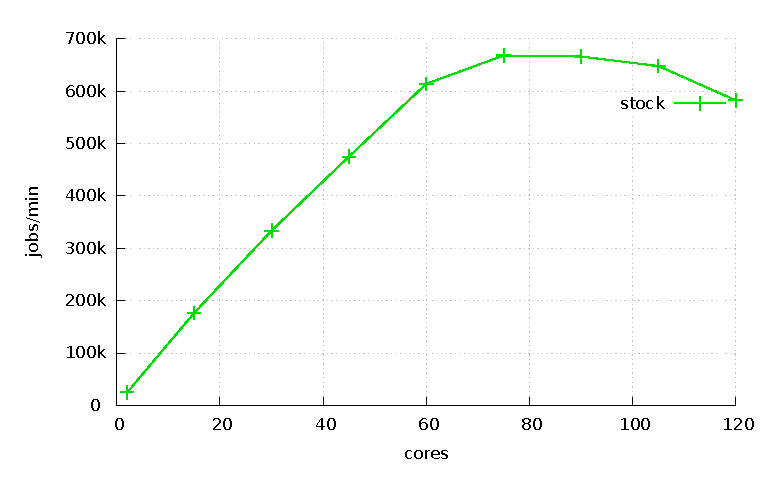
\includegraphics[width=\textwidth]{graph/aim7_default}
    \caption{AIM7-multiuser scalability}
  \end{subfigure}%
  \begin{subfigure}{0.45\textwidth}
    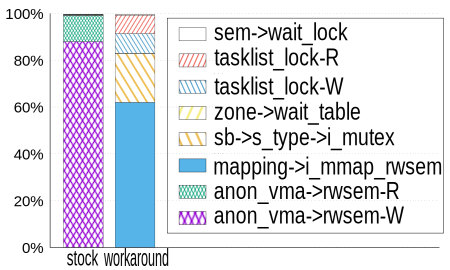
\includegraphics[width=\textwidth]{graph/lockstat}
    \caption{Lock wait time on 120 core}
  \end{subfigure}
  \centering
  \caption{Scalability of AIM7 multiuser and wait time to acquire locks on 120 core.
  This workload simultaneously create many processes. The (a) shows up to 75
  core, the stock Linux scales linearly, then it flattens out. The (b) left bar 
  represents anonymous reader-writer semaphore causes a scalability bottleneck, 
  and The (b) right bar shows file mapping reader-writer semaphore causes a
  scalability bottleneck.}
  \label{fig:aim7_default}
\end{figure}

Applications' performance would be limited by the operating system kernel when 
the operating system kernel does not scale well~\cite{Clements15SCR}~\cite{Boyd-WickizerCorey}.
%Linux has heavily optimized for multi-core operating systems.
To analyze the current status of the operating system scalability,
we measured the performance trends of the AIM7-multiuser benchmark on Linux
with various CPU cores.
The AIM benchmark has, until recently, been widely used in research area
and the Linux community~\cite{Bueso2015STP}~\cite{Bueso2014MCS}.
The AIM7-multiuser workload simultaneously creates many processes with
disk-file operations, virtual memory operations, pipe I/O, and arithmetic
operations.
%We used the temp filesystem to minimize the filesystem bottlenecks.
The result of figure~\ref{fig:aim7_default}(a) shows that
Linux shows significantly limited performance scalability when CPU core 
exceeds 75.

%$$$$$$$$$$$$$$$$$$$$$$$$$$$$$$$$$$$$$$$$$$$$$$$$$$$$$$$$$$$$$$$$$$$$$$$$$$$$$$$$
% Paragraph: Lockstat로 분석 결과 설명 
%$$$$$$$$$$$$$$$$$$$$$$$$$$$$$$$$$$$$$$$$$$$$$$$$$$$$$$$$$$$$$$$$$$$$$$$$$$$$$$$$

To understand the sources of scalability bottleneck on 120 core systems, we profiled a 
lock contention using the \code{lock\_stat}~\cite{LOCKSTAT}, a Linux kernel lock profiler that reports how
long each lock is held and the wait time to acquire the lock.
The figure~\ref{fig:aim7_default}(b) shows the cost of acquiring the lock for the AIM7-multiuser
running on a 120 core system.
Results of the \code{lock\_stat} that the main source of lock contention was the 
anonymous reverse mapping semaphore(\code{anon\_vma->rwsem}), 
which was caused by simultaneously creating a number of processes.
%The reverse page mapping records page information when using fork(), exit() and
%mmap() system call to find all page table entries.
To understand further bottlenecks, we intentionally removed the kernel codes causing 
anonymous reverse mapping which has been revealed as the most significant source of the problem.
%conducted a workaround by removing
%anonymous reverse mapping relative code in the part of the Linux fork with page-swap off
%because of avoiding the Linux page reclaiming.
When the anonymous reverse mapping code was removed, 
the second major source of the bottleneck was file 
reverse mapping reader-writer semaphore(\code{mapping->i\_mmap\_rwsem}).

%$$$$$$$$$$$$$$$$$$$$$$$$$$$$$$$$$$$$$$$$$$$$$$$$$$$$$$$$$$$$$$$$$$$$$$$$$$$$$$$$
% Paragraph : 리눅스 reverse page map의 write serialization 문제점
%$$$$$$$$$$$$$$$$$$$$$$$$$$$$$$$$$$$$$$$$$$$$$$$$$$$$$$$$$$$$$$$$$$$$$$$$$$$$$$$$

Our background study showed that both the anonymous reverse mapping
reported from the Linux community~\cite{Andi2011adding} and the file reverse mapping reported from S.
Boyd-Wickizer~\cite{SilasBoydWickizerPth} are significant factors in fork scalability problem.
Thus, in order to perfect scalability of the fork, both the
file reverse mapping and the anonymous reverse mapping should be executed
concurrently without any lock.
%In fact, the fundamental scalability problem of reverse mapping is their
%serialized update operations because operating systems are serialized at
%the update operations.

%$$$$$$$$$$$$$$$$$$$$$$$$$$$$$$$$$$$$$$$$$$$$$$$$$$$$$$$$$$$$$$$$$$$$$$$$$$$$$$$$
% Paragraph : update heavy한 상황에 대한 설명과 해결 방법에 대한 설명
%$$$$$$$$$$$$$$$$$$$$$$$$$$$$$$$$$$$$$$$$$$$$$$$$$$$$$$$$$$$$$$$$$$$$$$$$$$$$$$$$

Existing research accomplishments to achieve scalable concurrent update in many
core systems are categorized into two methods:
non-blocking
algorithms~\cite{Harris2001Lockfree}~\cite{Fomitchev2004Lockfree}~\cite{Timnat2012}
in early stages and log-based algorithms.
In non-blocking algorithms, update operation observes against the current
value in global data structure, and they execute an atomic compare and swap(CAS) to 
compare the against value.
When the value has been overridden, the updater must be retried.
Consequently, both the repeated global CAS operation and the iteration loop caused
by CAS fails will result in bottlenecks due to inter-core communication
overheads~\cite{SilasBoydWickizerPth}.
To overcome the problem of cache coherence systems, log-based methods are
proposed.
%Our research also uses a log-based deferred design that alows concurrent
%updates to scale, so that multiprocessed applications can scale to large
% numbers of cores.

%$$$$$$$$$$$$$$$$$$$$$$$$$$$$$$$$$$$$$$$$$$$$$$$$$$$$$$$$$$$$$$$$$$$$$$$$$$$$$$$$
%Paragraph : Log 기반의 알고리즘 대략적인 설명 
%$$$$$$$$$$$$$$$$$$$$$$$$$$$$$$$$$$$$$$$$$$$$$$$$$$$$$$$$$$$$$$$$$$$$$$$$$$$$$$$$

%Log-based algorithm is that when update operations occur, it logs the update
%operation and applies the all operation logs to the data structure
%before read operation, so reader can read up to date data structure.

The log-based algorithms are
a suitable solution for the update-heavy data structure because they allow
update operations to proceed with a coarse-grained update lock or without
update locks.
The benefit of avoiding a fine-grained update lock can eliminate the overhead of
acquiring a lock that requires fetching the lock's cache line.
Thus, it reduces the cache communication traffic;a contended cache line on
many-core processors can take hundreds of cycles to fetch from a remote
core~\cite{AustinTClements2012RCUBalancedTrees}, and these techniques can be easily applied to other data structures.
%In addition to avoiding fine-grained lock and easily applying the
%other data structures, a log-based method can remove an existing
%operation log rather than actually executing a operation log.

One notable recent research accomplishment regarding log-based approach is
the OpLog proposed by S. Boyd-Wickizer \textit{et al.}.
The OpLog utilizes representative distributed systems management concepts(e.g., Google spanner's 
synchronized clocks scheme~\cite{Corbett2013SGG}) and proposes the log-based algorithm to shared-memory systems.
The OpLog shows significant improvement in performance scalability for update-heavy operating system
data structures.
Though the OpLog forms an important basis for another step of improvement in performance
scalability problem in many core systems, it still has limitation that it's 
synchronized time-stamp counters might cause additional overhead during log management
process.
%The OpLog using the synchronized time-stamp counters method may incur
%time-stamp merging and ordering process.
%Consequently, when core counts increases, the time-stamp merging and ordering
%process may require sequential processing, which can limit scalability and
%performance.
%For example, if cores counts are 1000 and per-core logs counts are 10, 
%because each log searches all core's log, 